\documentclass[tikz,border=8pt]{article}
\usepackage{graphicx} 
\usepackage{amsfonts}
\usepackage{mathtools}
\usepackage{amssymb}
\usepackage{tcolorbox}
\usepackage{algorithm}
\usepackage{algpseudocode}
\usepackage{quantikz}
\usepackage{amsmath}
\usepackage{hyperref}
\usepackage{tikz}
\usetikzlibrary{positioning,arrows.meta,decorations.pathmorphing,shadings}

\title{Quantum Walks}
\author{Riccardo Marega}
\date{December 2025}

\begin{document}
\maketitle
\tableofcontents
\newpage
\section{Introduction}
\subsection{Graph theory}
\paragraph{Graph $\left(G\right)$:} ordered triple $\left( \mathbf{V}\left(G\right),\mathbf{E}\left(G\right),\psi_G \right)$ consisting of a nonempty set $\mathbf{V}\left(G\right)$ of vertices, a set $\mathbf{E}\left(G\right)$, disjoint from $\mathbf{V}\left(G\right)$, of edges, and an incidence function $\psi_G$ that associates with each edge of G an unordered pair of (not necessarily distinct) vertices of G.\\
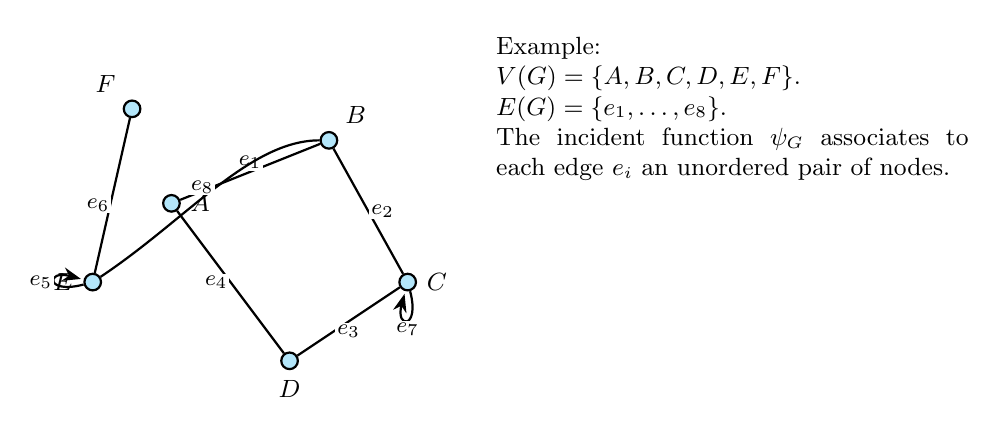
\begin{tikzpicture}[>=Stealth, every node/.style={font=\small}]
\tikzset{
  mynode/.style={
    draw,
    circle,
    fill=cyan!30,
    inner sep=1.8pt,
    minimum size=6pt,
    thick,
    label distance=2mm,
  },
  edgelabel/.style={font=\footnotesize, fill=white, inner sep=0.7pt}
}
\node[mynode, label=right:{$A$}] (A) at (0,0) {};
\node[mynode, label=above right:{$B$}] (B) at (2,0.8) {};
\node[mynode, label=right:{$C$}] (C) at (3,-1) {};
\node[mynode, label=below:{$D$}] (D) at (1.5,-2) {};
\node[mynode, label=left:{$E$}] (E) at (-1,-1) {};
\node[mynode, label=above left:{$F$}] (F) at (-0.5,1.2) {};
\draw[thick] (A) -- (B) node[midway, above, edgelabel] {$e_1$};
\draw[thick] (B) -- (C) node[midway, right, edgelabel] {$e_2$};
\draw[thick] (C) -- (D) node[midway, below, edgelabel] {$e_3$};
\draw[thick] (D) -- (A) node[midway, left, edgelabel] {$e_4$};
\draw[thick] (B) .. controls (1,0.8) and (0.2,-0.2) .. (E) node[midway, left, edgelabel] {$e_8$};
\draw[thick] (E) -- (F) node[midway, below left, edgelabel] {$e_6$};
\path[thick] (E) edge[loop left] node[left, edgelabel] {$e_5$} (E);
\path[thick] (C) edge[loop below] node[below, edgelabel] {$e_7$} (C);
\node[anchor=west] at (4.0,1.2) {\begin{minipage}{6cm}
\small
Example:
\\
$V(G)=\{A,B,C,D,E,F\}$.\\
$E(G)=\{e_1,\dots,e_8\}$.\\
The incident function $\psi_G$ associates to each edge $e_i$ an unordered pair of nodes.
\end{minipage}};
\end{tikzpicture}
\newline
Let $\mathbf{Y}$ be a random variable over a finite space $\mathbf{X} \subseteq \mathbb{R}^d$, with $|\mathbf{X}|=n$ and $d\geq1$.\\
For $y \in \mathbf{X}$, we denote $Pr\left(Y=y\right)$ as the probability that $Y = y$.\\
A sequence of random variables $\mathbf{Y} = (Y_t)^{\infty}_{t=0}$ over $\mathbf{X}$ is a \textbf{Markov chain} if for all $t\geq 1,$ $Y_t$ is independent of $Y_0,\cdots,Y_{t-2}$ given $Y_{t-1}$,i.e.: $$
Pr\left(Y_{t} = y_t|Y_{t-1} = y_{t-1},\cdots,Y_1 = y_1\right) = Pr\left(Y_{t} = y_t|Y_{t-1} = y_{t-1}\right) \eqqcolon P_t\left(y_{t-1},y_t\right)$$
with
$$ 
y_1,\cdots,y_t \in \mathbf{X},
$$\\
where $P_t\left(x,y\right)$ is the one-step transition probability from the state $x$ to the state $y$ at the time step $t$.\\
The chain is \textbf{time-homogeneous} when $P_t = P$ $\forall t\geq1$.\\
A \textbf{stationary time-homogeneous} chain is characterized by the same marginal distribution $\mathbf{Y}_t$ for every $t$, i.e. the distribution $\pi$ of $\mathbf{Y}_t$ is invariant under the transition matrix $P$:
$$
\pi P = \pi.
$$
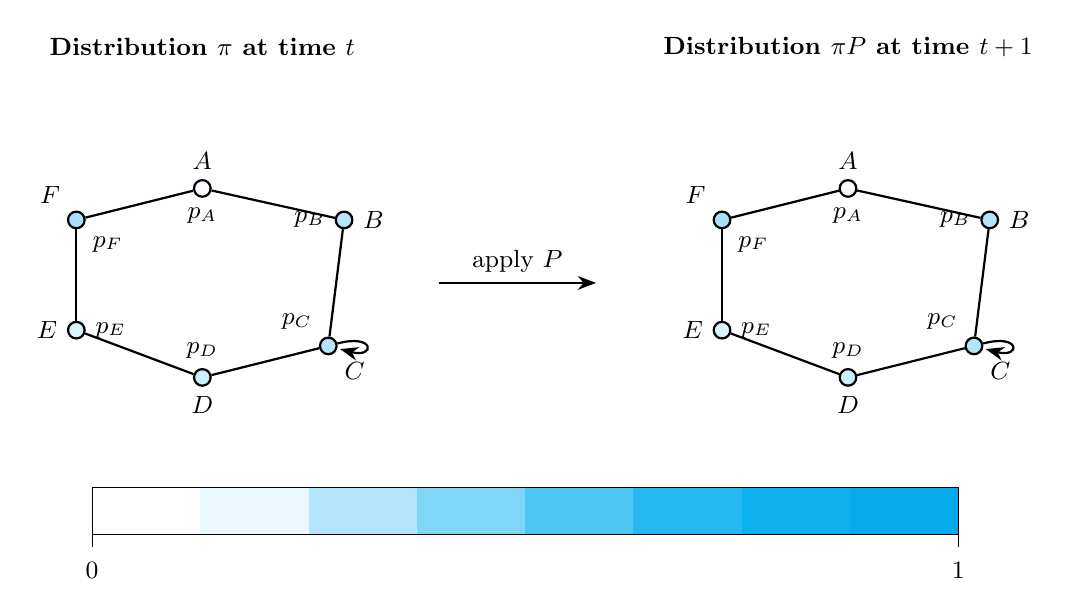
\begin{tikzpicture}[>=Stealth, every node/.style={font=\small}]
\tikzset{
  sA/.style={circle, draw, fill=cyan!2,  minimum size=6pt, thick,inner sep=1.8pt},
  sB/.style={circle, draw, fill=cyan!30, minimum size=6pt, thick,inner sep=1.8pt},
  sC/.style={circle, draw, fill=cyan!30, minimum size=6pt, thick,inner sep=1.8pt},
  sD/.style={circle, draw, fill=cyan!20, minimum size=6pt, thick,inner sep=1.8pt},
  sE/.style={circle, draw, fill=cyan!15, minimum size=6pt, thick,inner sep=1.8pt},
  sF/.style={circle, draw, fill=cyan!35, minimum size=6pt, thick,inner sep=1.8pt},
  edgelabel/.style={font=\scriptsize, fill=white, inner sep=0.6pt}
}
\node at (0,3.0) {\textbf{Distribution $\pi$ at time $t$}};
\node[sA, label=above:$A$, label=below:$p_A$] (A1) at (0,1.2) {};
\node[sB, label=right:$B$, label=left:$p_B$] (B1) at (1.8,0.8) {};
\node[sC, label=below right:$C$, label=above left:$p_C$] (C1) at (1.6,-0.8) {};
\node[sD, label=below:$D$, label=above:$p_D$] (D1) at (0,-1.2) {};
\node[sE, label=left:$E$, label=right:$p_E$] (E1) at (-1.6,-0.6) {};
\node[sF, label=above left:$F$, label=below right:$p_F$] (F1) at (-1.6,0.8) {};
\draw[thick] (A1) -- (B1);
\draw[thick] (B1) -- (C1);
\draw[thick] (C1) -- (D1);
\draw[thick] (D1) -- (E1);
\draw[thick] (E1) -- (F1);
\draw[thick] (F1) -- (A1);
\draw[->, thick] (C1) edge[loop right] (C1);
\draw[thick, ->] (3.0,0) -- (5.0,0)
node[midway, above] {\small apply $P$};
\node at (8.2,3.0) {\textbf{Distribution $\pi P$ at time $t+1$}};
\node[sA, label=above:$A$, label=below:$p_A$] (A2) at (8.2,1.2) {};
\node[sB, label=right:$B$, label=left:$p_B$] (B2) at (10.0,0.8) {};
\node[sC, label=below right:$C$, label=above left:$p_C$] (C2) at (9.8,-0.8) {};
\node[sD, label=below:$D$, label=above:$p_D$] (D2) at (8.2,-1.2) {};
\node[sE, label=left:$E$, label=right:$p_E$] (E2) at (6.6,-0.6) {};
\node[sF, label=above left:$F$, label=below right:$p_F$] (F2) at (6.6,0.8) {};
\draw[thick] (A2) -- (B2);
\draw[thick] (B2) -- (C2);
\draw[thick] (C2) -- (D2);
\draw[thick] (D2) -- (E2);
\draw[thick] (E2) -- (F2);
\draw[thick] (F2) -- (A2);
\draw[->, thick] (C2) edge[loop right] (C2);
\begin{scope}[shift={(-2,-3.2)}]
  \fill[white] (0.6,0) rectangle ({0.6+1.375},0.6);
  \foreach \i/\perc in {0/8, 1/30, 2/50, 3/70, 4/85, 5/95} {
    \fill[cyan!\perc] ({0.6+1.375+\i*1.375},0) rectangle ({0.6+1.375+(\i+1)*1.375},0.6);
  }
  \fill[cyan!98!black] ({0.6+1.375+6*1.375},0) rectangle (11.6,0.6);
  \draw (0.6,0) rectangle (11.6,0.6);
  \draw (0.6,0) -- ++(0,-0.15) node[below,yshift=-2pt] {\small $0$};
  \draw (11.6,0) -- ++(0,-0.15) node[below,yshift=-2pt] {\small $1$};
\end{scope}
\end{tikzpicture}
A time-homogeneous Markov chain on a finite time horizon $\left(Y_t\right)^N_{t=0}$ with transition matrix $P$ and stationary distribution $\pi$ is said to be \textbf{reversible} if $$
P^*(x,y) = \frac{\pi\left(y\right)P\left(y,x\right)}{\pi\left(x\right)} = P(x,y) \Rightarrow \pi\left(x\right)P\left(x,y\right)=\pi\left(y\right)P\left(y,x\right)
$$\\
for all $x,y \in \mathbf{X}$ given $\pi\left(x\right)>0$\footnote{This assumption is necessary for this construction.} for all $x \in \mathbf{X}$ and where $P^*(x,y)$ refers to the transition probabilities of the reversed chain $\left(Y_t\right)^0_{N}$.\\
In matrix form:$$
P^* = diag\left(\pi\right)^{-1}P^Tdiag\left(\pi\right).
$$
In other words, a Markov chain is reversible when its behavior in time is indistinguishable from that observed when time is run backward.\\
\paragraph{Theorem:} Given a stationary Markov chain $\mathbf{Y} = \left(Y_t\right)$ with $t\geq0$ on a finite space $\mathbf{X}$, with transition matrix $P$ and stationary distribution $\pi$, then the following statements hold:\begin{enumerate}
    \item \textbf{Detailed balance}: $\pi\left(x\right)P\left(x,y\right)=\pi\left(y\right)P\left(y,x\right)$ $\forall x,y \in \mathbf{X}$;
    \item \textbf{Two-step symmetry}: $Pr\left(Y_1 = y_1, Y_2 = y_2\right) = Pr\left(Y_1 = y_2, Y_2 = y_1\right)$\\$\forall y_1,y_2 \in \mathbf{X}$;
    \item \textbf{Finite-path symmetry}: $Pr\left(\left(Y_t\right)^N_0 = \left(y_t\right)^N_0\right) = Pr\left(\left(Y_t\right)^0_N = \left(y_t\right)^0_N\right)$\\$\forall\left(y\right)^N_0\in\mathbf{X}^N.$
\end{enumerate}
The chain is reversible if and only if any of these conditions (and therefore all conditions) hold.\\
\newline
A graph $G$ is a \textbf{bipartite} graph with vertex class $V_1$ and $V_2$ if $V(G) = V_1 \cup V_2, V_1 \cap V_2 = \varnothing$ and every edge joins a vertex of $V_1$ to a vertex of $V_2$.\\
Similarly $G$ is r-partite with vertex classes $V_1,\cdots,V_r$ if $V(G) = V_1 \cup\cdots\cup V_r, V_1\cap\cdots\cap V_r = \varnothing$, and no edges joins vertices in the same class.\\
Follows a graphical example:\\
\newline
\begin{center}
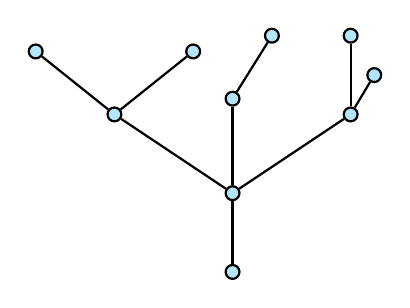
\begin{tikzpicture}[>=Stealth, every node/.style={font=\small}]
\tikzset{
  mynode/.style={
    draw,
    circle,
    fill=cyan!30,
    inner sep=1.5pt,
    minimum size=5pt,
    thick,
  }
}

\node[mynode] (A) at (0,0) {};
\node[mynode] (B) at (-1.5,1) {};
\node[mynode] (C) at (0,1.2) {};
\node[mynode] (D) at (1.5,1) {};
\node[mynode] (E) at (0,-1) {};
\node[mynode] (F) at (-2.5,1.8) {};
\node[mynode] (G) at (-0.5,1.8) {};
\node[mynode] (H) at (0.5,2) {};
\node[mynode] (I) at (1.5,2) {};
\node[mynode] (J) at (1.8,1.5) {};
\draw[thick] (A) -- (B);
\draw[thick] (A) -- (C);
\draw[thick] (A) -- (D);
\draw[thick] (A) -- (E);

\draw[thick] (B) -- (F);
\draw[thick] (B) -- (G);

\draw[thick] (C) -- (H);

\draw[thick] (D) -- (I);
\draw[thick] (D) -- (J);

\end{tikzpicture}
\end{center}
\subsection{Random walks}
A random walk on a graph is defined by a sequence of nodes, starting from a source node. At each step, the walker moves along an edge to a neighboring node, reaching a new node and repeating the process.\\
\newline
Given a weighted, undirected graph $\mathrm{G} = \left( \mathbf{X}\left(\mathrm{G}\right), \mathbf{E}\left(\mathrm{G}\right), \textit{w}\right)$ with $|\mathbf{X}| = n$, $\mathbf{E}\left(\mathrm{G}\right) \subset \mathbf{X} \times \mathbf{X}$ (such that $\left( u,v\right) \in \mathbf{E}$ if and only if $\left(v,u\right) \in \mathbf{E}$) and $\textit{w}:\mathbf{E} \rightarrow \mathbb{R}_{\geq 0}$\footnote{If an edge is not present then its weight is equal to zero, moreover the total weight is $\sum_{u,v \in \mathbf{X}}\textit{w}_{u,v}$ and the weight of the edges leaving a node $u$ is $\sum_{v\in \mathbf{X}}\textit{w}_{u,v}$.}, then a \textbf{Random Walk} on $\mathrm{G}$ is described by a Markov chain over $\mathbf{X}$ with \textbf{Transition Matrix} ($P$), defined by: $$
P_{u,v} = \frac{\textit{w}_{u,v}}{\sum_{v\in \mathbf{X}}\textit{w}_{u,v}}.
$$
In a random walk the choice of the following node $v$, given the current node $u$, is proportional to the edge weight $w_{u,v}$.\\
More precisely, a random walk on $\mathrm{G}$ is described by a reversible Markov chain.\\
If the graph is connected and non-bipartite, the random walk is said to be \textbf{ergodic} and its probability distribution \underline{converges} to the stationary distribution $\pi \in \mathbb{R}^d$ defined as: $$
\pi_u = \frac{\sum_{v\in \mathbf{X}}\textit{w}_{u,v}}{\sum_{u,v \in \mathbf{X}}\textit{w}_{u,v}} = \frac{w_u}{W}.
$$
$\pi$ is the only eigenvector of P with eigenvalue 1.\\
\newline
While the transition matrix $P$ of a reversible Markov chain is not always symmetric, the \textbf{Discriminant matrix} $D(P)$, defined using the transition matrix itself, is always symmetric:
$$
D(P) = diag(\sqrt{\pi})Pdiag(\sqrt{\pi})^{-1}.
$$
\subsubsection{Frameworks}...
\section{Quantum walks and quantum search algorithms}
\subsection{Preliminaries}
\paragraph{Lemma \textit{(Effective Spectral Gap)}.} Let $\Pi_A$ and $\Pi_B$ be two orthogonal projectors in the same vector space, and $R_A = 2\Pi_A - \mathbf{1}$ and $R_B = 2\Pi_B - \mathbf{1}$ be the reflection about their images. Assume $P_{\Theta}$, where $\Theta \geq 0$, is the orthogonal projector on the span of eigenvectors of $R_AR_B$ with eigenvalues $e^{i\theta(\beta)}$ such that $|\theta|\leq \Theta$ ($P_{\Theta} = \sum_{\beta:|\theta(\beta)|\leq \Theta}|\beta\rangle\langle\beta |$), where $\{|\beta\rangle\}$ is a complete orthonormal set of eigenvectors of $R_AR_B$. Then, for any vector $w$ in the kernel of $\Pi_B$ ($\Pi_B|w\rangle = 0$), we have $$
||P_{\Theta}\Pi_A|w\rangle||\leq\frac{\Theta}{2}|||w\rangle||.
$$
\newline
\textit{proof.} Let $|v\rangle = P_{\Theta}\Pi_A|w\rangle$, $|v'\rangle = R_B|v\rangle$ and $|v''\rangle = R_A|v'\rangle = R_AR_B|v\rangle$.\\
When $\Theta$ is small, $|v\rangle$ and $|v''\rangle$ are close:
$$
|| |v\rangle -|v''\rangle||^2 = ||\sum_{\beta:|\theta(\beta)|\leq\Theta}(1-e^{i\theta(\beta)}\langle\beta|v\rangle|\beta\rangle)||^2 \leq2(1-cos(\Theta))|||v\rangle||^2\leq\Theta^2|||v\rangle||^2.
$$
Notice that $|v\rangle+|v'\rangle$ is fixed by $R_B$. Similarly, $R_A$ fixes $|v'\rangle+|v''\rangle$ and $\bar{R}_A = \mathbf{1}-R_A$ fixes $|v'\rangle-|v''\rangle$.\\
Hence $0 = \langle v+v'|w\rangle = \langle v+v'|R_A|w\rangle + \langle v+v'|\bar{R}_A|w\rangle = \langle v+v''|R_A|w\rangle + \langle v-v''|\bar{R}_A|w\rangle$, therefore:\\
$|||v\rangle||^2 = |\langle v|R_A|w\rangle| = \frac{1}{2}|\langle v-v'|R_A|w\rangle + \langle v+v''|R_A|w\rangle| = \frac{1}{2}|\langle v-v''|(R_A-\bar{R}_A)|w\rangle|.$\\
We conclude $$
|||v\rangle||^2 \leq \frac{1}{2}|||v\rangle - |v''\rangle||||(R_A-\bar{R}_A)|w\rangle||\leq\frac{\Theta}{2}|||v\rangle||||w\rangle||.
$$
\hfill $\square$\\
\newline
\paragraph{Interpretation:}\textit{When the initial state is (approximately) orthogonal to one of the subspaces defining the reflections, the portion of the state supported on eigenvalues close to $1$ (i.e., eigenvectors nearly unaffected by rotation) is necessarily small. The lemma ensures that most of the state must therefore lie in spectral regions where $R_AR_B$ acts non-trivially, forcing the evolution to change the state rather than leaving it nearly fixed. In particular, the inequality shows that the non-evolving component is bounded by $\Theta/2$, meaning the part that remains almost unchanged is itself limited by $\Theta$.}
\subsubsection{Quantum Fourier Transform and Phase Estimation}
\paragraph{Motivation:} One of the most useful way of solving complex mathematical problems is to transforming them into problems for which the solutions are known.
\paragraph{Discrete Fourier Transform:}
$$
y_k = \frac{1}{\sqrt{N}}\sum_{j=0}^{N-1}x_je^\frac{2\pi ijk}{N},
$$
where the input vector $(x_0,\cdots,x_{N_1} )$ is a vector of length $N$ composed of complex numbers.
\paragraph{Quantum Fourier Transform:}$$
|j\rangle \rightarrow \frac{1}{\sqrt{N}}\sum_{j=o}^{N-1}e^{\frac{2\pi ijk}{N}}|k\rangle,
$$
where $\{|0\rangle,\cdots, |N-1\rangle\}$ constitute an orthonormal basis.\\
Equivalently, the action on an arbitrary state may be written as:$$
\sum_{j=0}^{N-1}x_j|j\rangle \rightarrow \sum_{k=0}^{N-1}y_k|k\rangle,
$$
where the amplitudes $y_k$ are the discrete Fourier transform of the amplitudes $x_j$.\\
\textit{It is not obvious from the definition, but this transformation is unitary and thus can be implemented as the dynamics for a quantum computer.}\\
The Fourier Transform is the key to a general procedure known as \textbf{phase estimation}, which in turn is the key for many quantum algorithms.\\
Suppose a unitary operator $U$ has an eigenvector $\psi$ with eigenvalue $e^{2 \pi i \phi}$, where the value of $\phi$ is unknown, phase estimation algorithm can be used to retrieve (or estimate) that value. To perform the estimation we assume that we have a black box (\textbf{oracle}) capable of preparing the state $|\psi\rangle$ and performing the controlled-$U^{2^j}$ operation, for suitable non-negative integers $j$. The use of black boxes indicates that phase estimation procedure is not a complete quantum algorithm in its own right (it rather have to be thought as a subroutine of more complex computational operations).\\
The quantum phase estimation procedure uses two registers. The first register contains $t$ qubits in the state $|0\rangle$ (where $t$ depends on the number of digits of accuracy we wish to have in the estimate for $\phi$ and with what probability we wish the phase estimation to be successful) and the second register begins in the state $|\psi\rangle$.\\
The phase estimation is performed in two stages: first the following circuit is applied
$$
\tikzset{every node/.append style={inner sep=1pt}}
{\scriptsize 
\begin{quantikz}[column sep=4pt, row sep=4pt, scale=0.88, transform shape]
\lstick[wires=4]{First register\\$t$ qubits} \ket{0} & \gate{H} & \qw & \qw & \qw & \qw \ldots \qw & \ctrl{4} & \qw & \rstick{$e^{2\pi i(2^{t-1}\varphi)}\ket{1}$} \\
\ket{0} & \gate{H} & \qw & \qw & \ctrl{3} & \qw \ldots \qw & \qw        & \qw & \rstick{$e^{2\pi i(2^{2}\varphi)}\ket{1}$} \\
\ket{0} & \gate{H} & \qw & \ctrl{2} & \qw        & \qw \ldots \qw & \qw        & \qw & \rstick{$e^{2\pi i(2^{1}\varphi)}\ket{1}$} \\
\ket{0} & \gate{H} & \ctrl{1} & \qw & \qw        & \qw \ldots \qw & \qw        & \qw & \rstick{$e^{2\pi i(2^{0}\varphi)}\ket{1}$} \\
\lstick{Second register\\$\ket{\psi}$}
        & \qw & \gate{U^{2^0}} & \gate{U^{2^1}} & \gate{U^{2^2}} & \qw \ldots \qw & \gate{U^{2^{t-1}}} & \qw & \rstick{\ket{\psi}}
\end{quantikz}
}
$$
then, the inverse of the quantum Fourier transform is applied to the first register.\\
The final state of the first register after having applied the previous circuit is:
$$
\frac{1}{2^{\frac{t}{2}}}\left[\left(|0\rangle + e^{2\pi i 2^{t-1}\phi}|1\rangle\right)\otimes\left(|0\rangle + e^{2\pi i 2^{t-2}\phi}|1\rangle\right)\otimes\cdots\otimes\left(|0\rangle + e^{2\pi i 2^{0}\phi}|1\rangle\right)\right] =
$$
$$
=\frac{1}{2^{\frac{t}{2}}}\sum_{k=0}^{2^t-1}e^{2\pi i \phi k}|k\rangle.
$$\footnote{Physical interpretation (useful for understanding the physical meaning of the iQFT):\begin{itemize}
    \item $k$ is the discrete "time/position" index,  
    \item $\phi$ is the frequency (or wave number),  
    \item $e^{2 \pi i \phi k}$ represents a periodic oscillation.

\end{itemize}}
The previous computation can be found in \hyperref[app:A]{\textit{Appendix A}}.\\
After having then applied the inverse quantum transform to the first register $$
\frac{1}{2^{\frac{t}{2}}}\sum_{j=0}^{2^t-1}e^{2\pi i \phi k}|k\rangle\otimes|\psi\rangle \rightarrow |\tilde{\phi}\rangle\otimes|\psi\rangle,
$$
where $|\tilde{\phi}\rangle$ is a good estimator for $\phi$, the final step is to read the output of first register by performing a measurement in the computational basis:
$$
|\tilde{\phi}\rangle \rightarrow \tilde{\phi}.
$$
As noted in the last section, in the case $\phi = 0.a_1\cdots a_t$, the state $|a_1\cdots a_t\rangle$ (hence $\phi$) can be obtained by just applying the inverse of the \textit{QFT}. This will produce the state $|a_1\cdots a_t\rangle$ exactly, however, in case $\phi$ is not a fraction of a power of two, applying the inverse of the \textit{QFT} produces the best m-bit approximation of $\phi$ with probability at least $\frac{4}{\pi^2}=0.405\cdots .$\\
To see why, let $\frac{a}{2^t} = 0.a_1\cdots a_t$ be the best m-bit estimate of $\phi$. Then $\phi = \frac{a}{2^t}+\delta$, where $0\leq |\delta |\leq\frac{1}{2^{t+1}}$. Applying the inverse \textit{QFT} to the state $$
\frac{1}{2^{\frac{t}{2}}}\left[\left(|0\rangle + e^{2\pi i 2^{t-1}\phi}|1\rangle\right)\otimes\left(|0\rangle + e^{2\pi i 2^{t-2}\phi}|1\rangle\right)\otimes\cdots\otimes\left(|0\rangle + e^{2\pi i 2^{0}\phi}|1\rangle\right)\right] =
$$
$$
=\frac{1}{2^{\frac{t}{2}}}\sum_{k=0}^{2^t-1}e^{2\pi i \phi k}|k\rangle,
$$
yields the state
$$
\frac{1}{2^t}\sum_{j=0}^{2^t-1}\sum_{k=0}^{2^t-1}e^{-\frac{2 \pi i j k}{2^m}}e^{2 \pi i \phi k}|j\rangle = \frac{1}{2^t}\sum_{j=0}^{2^t-1}\sum_{k=0}^{2^t-1}e^{-\frac{2 \pi i j k}{2^m}}e^{2 \pi i (\frac{a}{2^m}+\delta) k}|j\rangle = 
$$
$$
= \frac{1}{2^t}\sum_{j=0}^{2^t-1}\sum_{k=0}^{2^t-1}e^{-\frac{2 \pi i (a-j) k}{2^m}}e^{2 \pi i \delta k}|j\rangle
$$
and the coefficient of $|a_1\cdots a_t\rangle = |a\rangle$, which can be computed when $j = a$\footnote{$\frac{1}{2^t}\sum_{j=0}^{2^t-1}\sum_{k=0}^{2^t-1}e^{-\frac{2 \pi i (a-j) k}{2^m}}e^{2 \pi i \delta k}|j\rangle$ $\rightarrow_{j=a}$ $\frac{1}{2^t}\sum_{k=0}^{2^t-1}e^{2 \pi i \delta k}|a\rangle$}, in the above is the geometric series
$$
\frac{1}{2^t}\sum_{k=0}^{2^t-1}(e^{2 \pi i \delta})^k = \frac{1}{2^t}\left(\frac{1-(e^{2 \pi i \delta})^{2^t}}{1-e^{2 \pi i \delta}}\right).
$$
Since $|\delta| \leq \frac{1}{2^{t+1}}$, it follows that $2 \pi \delta 2^t \leq \pi$, and thus $|1-e^{2 \pi i \delta 2^t}| \geq \frac{2 \pi \delta 2^t}{\frac{\pi}{2}} = 4 \delta 2^t$. Also, $|1-e^{2 \pi i \delta}| \leq 2 \pi \delta$. Therefore, the probability of observing $a_1\cdots a_t$ when measuring the state is $$
\left| \frac{1}{2^m}\left( \frac{1-(e^{2 \pi i \delta})^{2^m}}{1-e^{2 \pi i \delta}}\right)\right|^2 \geq \left( \frac{1}{2^m} \left( \frac{4\delta 2^m}{2 \pi \delta}\right)\right) ^2 = \frac{4}{\pi^2}.
$$
The success probability can be amplified to $1 -\epsilon$ for any $\epsilon >0$ by inflating $t$ to $t^{'} = t + \mathbb{O}\left(\log\left( \frac{1}{\epsilon}\right)\right)$, and rounding off the resulting $t^{'}$-bit string to its most significant $t$ bits.
\paragraph{\textcolor{red}{Theorem \textit{(Phase estimation)}}.} \textcolor{red}{Assume a unitary $U$ is given as a black box. There exist a quantum algorithm that, given an eigenvector $\psi \in U$ with eigenvalue $e^{i\phi}$, outputs a real number $w$ such that $|w-\phi|\leq\delta$ with probability at least $\frac{9}{10}$. Moreover, the algorithms uses $\mathbb{O}(\frac{1}{\delta})$ controlled applications of $U$ and $\frac{1}{\delta}polylog\left(\frac{1}{\delta}\right)$ other elementary operations.}\\
\newline
\textit{\textcolor{red}{proof.}} \textcolor{red}{...}\\
\newline
\subsection{Quantum walk}
\paragraph{Definition \textit{(Quantum walk operator).}} For any reversible Markov chain $P$ on a finite state space $X$, a \textbf{quantum walk operator} $W(P)$ is a unitary $\mathit{H}_A\otimes\mathit{H_X}$, such that $|\bar{0}\rangle \in \mathit{H_A}$, $span\{|u\rangle:u\in X\} \subseteq \mathit{H_X}$, and for all $u \in X$ it holds that $$
\left(\langle \bar{0}|\otimes \langle u|\right)W\left(P\right)\left(| \bar{0}\rangle \otimes \mathbf{1}_X\right) = \langle u|D(P)
$$
\begin{center}
    and
\end{center}
$$
\left(\langle \bar{0}|\otimes \mathbf{1}_X\right)W\left(P\right)\left(| \bar{0}\rangle \otimes |u\rangle\right) = D(P)|u\rangle.
$$
\newline
In this framework, if $\mathit{H_u}$ denotes the \textit{local space} of $u$, $\bigoplus_{u\in\mathit{H_X}}\mathit{H_u}$ equals the whole space of the quantum walk, and $\bigoplus_{u\in\mathit{H_A}}\mathit{H_u}$ equals the residual subspace.\\
\newline
Defined as $\sigma$ the initial probability distribution, the quantum walk starts in the state $$
\varsigma = \sum_{\psi \in \mathit{H}_A\otimes\mathit{H_X}}\sqrt{\sigma_{\psi}}|\psi\rangle.
$$
The \textbf{step of the quantum walk} is defined by $R_AR_X$ where $R_X = \bigoplus_{u\in X}D_u$ and $R_A = \bigoplus_{u\in A}D_u$ are the direct sums of the diffusion operations. Each $D_u$ is a reflection operation in $\mathit{H}_u$. Hence, all $D_u$ in $R_X$ or $R_A$ commute, that makes them easy to implement in parallel. They are as follows:\begin{itemize}
    \item If $u$ is marked, then $D_u$ is the identity $\mathbf{1}_u$, i.e., the reflection about $\mathit{H_u}$;
    \item If $u$ in not marked, then $D_u$ is the reflection about the orthogonal component of $\psi_u \in \mathit{H_u}$, where $$
    |\psi_u\rangle = \sqrt{\frac{\sigma_u}{C_1R}}|u\rangle +\sum_{u,v \in \mathit{H_A}\otimes\mathit{H_X}}\sqrt{w_{uv}}|uv\rangle
    $$
    where $C_1 > 0$.
\end{itemize}
\paragraph{Note:} \textit{In the context of a quantum walk, the Effective Spectral Gap Lemma ensures that the state cannot remain trapped in the ``slow'' spectral regions. The portion of the state corresponding to eigenvalues near $1$ (almost unaffected by rotation) is bounded by $\Theta$, so most of the state lies in regions where $R_AR_X$ acts non-trivially. Each application of $R_AR_X$ moves the state significantly, guaranteeing progress through the walk. Moreover, a larger spectral gap implies faster evolution, preventing the walk from getting stuck in subspaces.}\\
\newline
\begin{tcolorbox}[colback=white,colframe=black,title={Quantum walk algorithm}]
\small
\begin{algorithm}[H]
\caption{}
\begin{algorithmic}[1]
\State Start in the state $\varsigma$.
\State Calculate, for each $u\in \mathit{H_A}\otimes\mathit{H_X}$, whether it is marked, and measure this bit.
\If {the result of the measurement shows `marked'}
    \State \textbf{output} ``marked vertices exist''.
    \State \textbf{quit}.
\EndIf
\State Execute quantum phase estimation on $R_A R_X$ with precision $\dfrac{1}{C\sqrt{RW}}$.
\If {the eigenvalue is $1$}
    \State \textbf{output} ``marked vertices exist''.
\Else
    \State \textbf{output} ``no marked vertices''.
\EndIf
\end{algorithmic}
\end{algorithm}
\end{tcolorbox}
\paragraph{Theorem} The previous algorithm detects the presence of a marked vertex with probability at least $\frac{2}{3}$. The algorithms uses $\mathbb{O}(\sqrt{RW})$ steps of the quantum walk.\\
\newline
\textit{proof} ...
\newpage
\appendix
\section{First half of the mathematical computation of the first register evolution in the phase estimation algorithm}\label{app:A}
Given $$
U^{2^j}|\psi\rangle = e^{2\pi i 2^j\phi}|\psi\rangle
$$
after having applied the \textit{H-gates} to the initial state we have:$$
|\Psi_1\rangle = (\textbf{H}^{\otimes^t} \otimes \textbf{1})[|0\rangle^{\otimes ^t} \otimes |\psi\rangle] =
$$
$$
= \frac{1}{2^{\frac{t}{2}}}\bigotimes_{j=1}^t(|0\rangle_j + |1\rangle_j)\otimes |\psi\rangle.
$$
Applying \textit{$C-U^{2^j} gates$} we have:
$$
\left(\prod_{m=1}^tC-U^{2^{t-m}}\right)|\Psi_1\rangle =
$$
$$
(C-U^{2^0})(C-U^{2^1})\cdots(C-U^{2^{t-2}})\underbrace{(C-U^{2^{t-1}})}_{|0\rangle_1\langle0|\otimes \textbf{1}_{2^{t-1}}\otimes \textbf{1} + |1\rangle_1\langle1|\otimes \textbf{1}_{2^{t-1}}\otimes \textbf{U}^{2^{t-1}}}|\Psi_1\rangle = 
$$
$$
(C-U^{2^0})(C-U^{2^1})\cdots(C-U^{2^{t-2}})(C-U^{2^{t-1}})\left[\frac{1}{2^{\frac{t}{2}}}\bigotimes_{j=1}^t\left(|0\rangle_j + |1\rangle_j \right)\otimes |\psi\rangle \right] =
$$
$$
(C-U^{2^0})(C-U^{2^1})\cdots(C-U^{2^{t-3}})\frac{1}{2^{\frac{t}{2}}}(|0\rangle_1+e^{2\pi i 2^{t-1}}|1\rangle_1)\otimes(|0\rangle_2+e^{2\pi i 2^{t-2}}|1\rangle_2)\otimes \left[\bigotimes_{j=3}^t\left(|0\rangle_j + |1\rangle_j \right)\otimes |\psi\rangle \right] =
$$
$$
\frac{1}{2^{\frac{t}{2}}}\bigotimes_{j=1}^t\left(|0\rangle_j + e^{2\pi i 2^{t-j}}|1\rangle_j \right)\otimes |\psi\rangle =
$$
$$
\frac{1}{2^{\frac{t}{2}}}\left[\left(|0\rangle + e^{2\pi i 2^{t-1}\phi}|1\rangle\right)\otimes\left(|0\rangle + e^{2\pi i 2^{t-2}\phi}|1\rangle\right)\otimes\cdots\otimes\left(|0\rangle + e^{2\pi i 2^{0}\phi}|1\rangle\right)\right] \otimes |\psi\rangle =
$$
$$
=\boxed{\frac{1}{2^{\frac{t}{2}}}\sum_{k=0}^{2^t-1}e^{2\pi i \phi k}|k\rangle \otimes |\psi\rangle.}
$$
\end{document}